\chapter{Antenna Theory Basics}
\label{ch:antenna-theory}

\begin{nontechnical}
\textbf{An antenna is like a funnel for radio waves}---it concentrates energy in one direction (transmit) or collects it from many directions (receive).

\textbf{Simple analogies}: - \textbf{Flashlight vs.~bare bulb}: A
flashlight (directional antenna) focuses light. A bare bulb
(omnidirectional) lights up everything. - \textbf{Satellite dish}:
Curved shape collects weak space signals and focuses them onto a tiny
receiver - \textbf{Your cell phone}: Has multiple tiny antennas
inside-\/-\/-cellular, WiFi, GPS, Bluetooth (each tuned to different
frequencies)

\textbf{Key insights}:
\begin{itemize}
\item \textbf{Bigger = stronger}: 10-meter dish collects 100$\times$ more energy than 1-meter dish
\item \textbf{Shape matters}: Long wire for AM radio, small stub for WiFi, dish for satellites
\item \textbf{Trade-off}: Omnidirectional (WiFi router) covers whole area but weak. Directional (satellite dish) is strong but must point exactly right.
\end{itemize}
\end{nontechnical}

\section{Overview}

An \textbf{antenna} is a transducer that converts \textbf{electrical signals into electromagnetic waves} (transmit) and vice versa (receive). Antennas are governed by \textbf{reciprocity}: their transmit and receive properties are identical.

\begin{keyconcept}
\textbf{Fundamental principle:} Accelerating charges radiate electromagnetic energy. This relationship, described by Maxwell's equations, forms the basis for all antenna operation. An antenna provides the interface between guided waves (on transmission lines) and free-space electromagnetic radiation.
\end{keyconcept}

The design and analysis of antennas spans multiple disciplines: electromagnetics, circuit theory, signal processing, and materials science. This chapter focuses on the fundamental parameters and design principles that apply across all antenna types.

\section{Mathematical Description}

\subsection{Power Density and Radiation}

The power density $S$ at distance $r$ from an isotropic radiator with transmit power $P_t$ is:
\begin{equation}
S_{\text{iso}} = \frac{P_t}{4\pi r^2}
\label{eq:power-density-iso}
\end{equation}
where:
\begin{itemize}
\item $S_{\text{iso}}$ = power density (W/m$^2$)
\item $P_t$ = transmit power (Watts)
\item $r$ = distance from antenna (meters)
\end{itemize}

For a directional antenna with gain $G$, the power density is enhanced:
\begin{equation}
S(\theta, \phi) = \frac{P_t G(\theta, \phi)}{4\pi r^2}
\label{eq:power-density-directional}
\end{equation}

\subsection{Effective Aperture and Received Power}

The effective aperture $A_e$ relates an antenna's gain to its equivalent capture area:
\begin{equation}
A_e = \frac{G \lambda^2}{4\pi}
\label{eq:effective-aperture}
\end{equation}
where $\lambda$ is the wavelength (meters).

The received power is then:
\begin{equation}
P_r = S \cdot A_e
\label{eq:received-power}
\end{equation}

\section{Key Antenna Parameters}

\subsection{1. Radiation Pattern}

\textbf{The spatial distribution of radiated power} describes how an antenna directs energy in three-dimensional space.

\textbf{Coordinate system:}
\begin{itemize}
\item \textbf{Azimuth ($\phi$)}: Horizontal angle (0$°$ to 360$°$)
\item \textbf{Elevation ($\theta$)}: Vertical angle from zenith (0$°$ = straight up)
\end{itemize}

\begin{center}
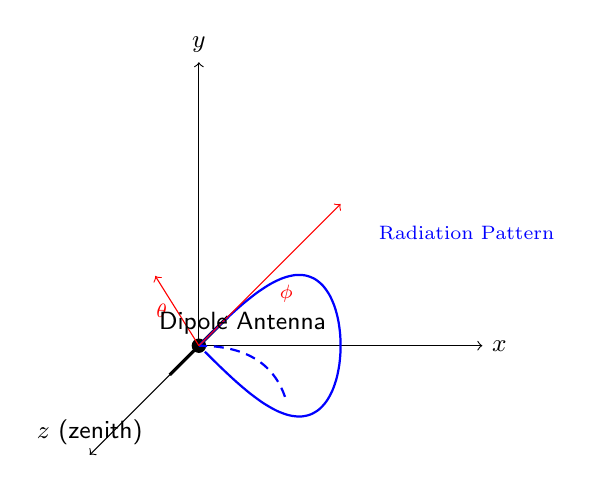
\begin{tikzpicture}[scale=1.2]
% Coordinate system
\draw[->] (0,0,0) -- (3,0,0) node[right] {\sffamily\small $x$};
\draw[->] (0,0,0) -- (0,3,0) node[above] {\sffamily\small $y$};
\draw[->] (0,0,0) -- (0,0,3) node[above] {\sffamily\small $z$ (zenith)};

% Dipole antenna
\draw[very thick,black] (0,0,-0.8) -- (0,0,0.8);
\filldraw[black] (0,0,0) circle (2pt);

% Radiation pattern (toroidal for dipole)
\draw[thick,blue] plot[smooth,domain=0:360,samples=60] ({1.5*abs(sin(\x))},{1.5*abs(sin(\x))*cos(\x)},{0});
\draw[thick,blue,dashed] plot[smooth,domain=0:180,samples=30] ({1.5*abs(sin(\x))},{0},{1.5*abs(sin(\x))*sin(\x)});

% Angle annotations
\draw[->,red] (0,0,0) -- (1.5,1.5,0) node[midway,below right,font=\scriptsize] {$\phi$};
\draw[->,red] (0,0,0) -- (0,1.2,1.2) node[midway,left,font=\scriptsize] {$\theta$};

% Labels
\node[below,font=\sffamily\small] at (0,0,-1.2) {Dipole Antenna};
\node[right,font=\scriptsize,blue] at (1.8,1.2,0) {Radiation Pattern};
\end{tikzpicture}
\end{center}

\textbf{Typical patterns:}

\subsubsection{Isotropic Radiator (Theoretical Reference)}

An isotropic radiator radiates \textbf{equally in all directions} (spherical pattern). While physically impossible to construct, it serves as the reference standard for antenna gain measurements.

The power density at distance $r$ from an isotropic source is given by Equation~\ref{eq:power-density-iso}.

\begin{calloutbox}{Note on Isotropic Reference}
The isotropic radiator is a theoretical construct used to define antenna gain in dBi (decibels relative to isotropic). All real antennas have some directivity, making them more efficient than an isotropic radiator in at least one direction.
\end{calloutbox}

\subsubsection{Half-Wave Dipole ($\lambda$/2)}

The \textbf{half-wave dipole} is the most fundamental practical antenna: a straight conductor with length equal to half the wavelength.

\textbf{Radiation pattern characteristics:}
\begin{itemize}
\item \textbf{Omnidirectional in azimuth} ($\phi$): Equal radiation in all horizontal directions
\item \textbf{Figure-8 in elevation} ($\theta$): Maximum broadside, nulls along wire axis
\item \textbf{3D pattern}: Donut-shaped (toroidal)
\end{itemize}

\textbf{Key parameters:}
\begin{equation}
R_r = 73\ \Omega
\label{eq:dipole-radiation-resistance}
\end{equation}
where $R_r$ is the radiation resistance for a lossless half-wave dipole.

The antenna gain relative to isotropic:
\begin{equation}
G_{\text{dipole}} = 2.15\ \text{dBi}
\label{eq:dipole-gain}
\end{equation}

\subsubsection{Directional Antennas}

High-gain antennas concentrate energy in specific directions through various mechanisms.

\textbf{Yagi-Uda antenna} (TV antenna):
\begin{itemize}
\item Single driven element (dipole)
\item Parasitic elements (directors + reflector)
\item \textbf{Gain}: 10--15 dBi
\item \textbf{Beamwidth}: $\sim$30--60$°$
\end{itemize}

\textbf{Parabolic dish:}
\begin{itemize}
\item Large aperture (diameter $D \gg \lambda$)
\item \textbf{Gain}: 30--60 dBi (satellite comms)
\item \textbf{Beamwidth}: $\theta \approx 70\lambda/D$ degrees
\end{itemize}

The beamwidth for aperture antennas can be approximated by:
\begin{equation}
\theta_{\text{HPBW}} \approx \frac{k\lambda}{D}
\label{eq:aperture-beamwidth}
\end{equation}
where $k \approx 70$ for parabolic reflectors and $\theta_{\text{HPBW}}$ is the half-power beamwidth in degrees.

\textbf{Phased array:}
\begin{itemize}
\item Multiple elements with controllable phase
\item \textbf{Electronically steerable} beam (no mechanical movement)
\item Used in: Radar, 5G base stations, THz communications
\end{itemize}

\subsection{2. Antenna Gain (G)}

Antenna gain quantifies the \textbf{ratio of power density in the preferred direction versus an isotropic radiator} with the same input power.

\begin{equation}
G(\theta, \phi) = \frac{S(\theta, \phi)}{S_{\text{iso}}}
\label{eq:antenna-gain}
\end{equation}

\textbf{Units}: dBi (decibels relative to isotropic)

\textbf{Typical gains}:

{\def\LTcaptype{} % do not increment counter
\begin{longtable}[]{@{}lll@{}}
\toprule\noalign{}
Antenna Type & Gain (dBi) & Beamwidth \\
\midrule\noalign{}
\endhead
\bottomrule\noalign{}
\endlastfoot
Isotropic (reference) & 0 dBi & 360\$\^{}\textbackslash circ\$ (all
directions) \\
Dipole (\$\textbackslash lambda\$/2) & 2.15 dBi &
\textasciitilde78\$\^{}\textbackslash circ\$ (elevation) \\
Monopole (\$\textbackslash lambda\$/4) & 5.15 dBi &
\textasciitilde30\$\^{}\textbackslash circ\$ (over ground plane) \\
Patch (microstrip) & 6-9 dBi &
\textasciitilde70-90\$\^{}\textbackslash circ\$ \\
Yagi (10 elements) & 12-15 dBi &
\textasciitilde30\$\^{}\textbackslash circ\$ \\
Parabolic dish (1 m @ 10 GHz) & \textasciitilde40 dBi &
\textasciitilde2\$\^{}\textbackslash circ\$ \\
Phased array (64 elements) & 18-24 dBi & Steerable \\
\end{longtable}
}

\textbf{Relationship to directivity:}
\begin{equation}
G = \eta_{\text{ant}} \cdot D
\label{eq:gain-directivity}
\end{equation}
where:
\begin{itemize}
\item $D$ = Directivity (power concentration factor, dimensionless)
\item $\eta_{\text{ant}}$ = Antenna efficiency (0.5--0.95 typical, accounts for ohmic losses)
\end{itemize}

\begin{warningbox}
Antenna efficiency $\eta_{\text{ant}}$ accounts for all losses: conductor resistance, dielectric losses, impedance mismatch, and surface roughness. At higher frequencies (millimeter-wave and THz), surface roughness becomes the dominant loss mechanism, significantly reducing efficiency.
\end{warningbox}

\subsection{3. Directivity (D)}

Directivity is the \textbf{power concentration factor} independent of losses:

\begin{equation}
D = \frac{4\pi}{\Omega_A}
\label{eq:directivity}
\end{equation}
where $\Omega_A$ is the \textbf{solid angle} of the main lobe (steradians).

For \textbf{narrow-beam antennas}, directivity can be approximated by:
\begin{equation}
D \approx \frac{41{,}253}{\theta_E \cdot \theta_H}
\label{eq:directivity-beamwidth}
\end{equation}
where:
\begin{itemize}
\item $\theta_E$ = Elevation plane beamwidth (degrees)
\item $\theta_H$ = Azimuth plane beamwidth (degrees)
\end{itemize}

\begin{calloutbox}{Example: High-Gain Dish Directivity}
\textbf{Given:} Beamwidth $\theta_E = \theta_H = 10°$

\textbf{Solution:}
\begin{equation}
D = \frac{41{,}253}{10 \times 10} = 412.53\ (\text{linear}) = 26.2\ \text{dBi}
\end{equation}

\textbf{Interpretation:} This antenna concentrates power 412 times more than an isotropic radiator in the beam direction.
\end{calloutbox}

\subsection{4. Beamwidth}

The \textbf{half-power beamwidth (HPBW)} is the angular width where the radiated power drops to half (-3 dB) of the peak value.

\begin{center}
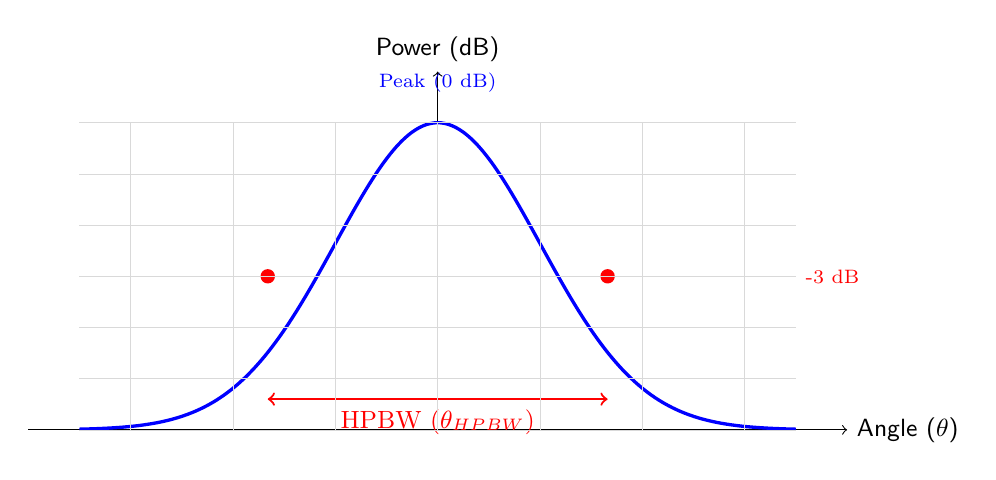
\begin{tikzpicture}[scale=1.3]
% Axes
\draw[->] (-4,0) -- (4,0) node[right] {\sffamily\small Angle ($\theta$)};
\draw[->] (0,0) -- (0,3.5) node[above] {\sffamily\small Power (dB)};

% Radiation pattern (Gaussian-like main lobe)
\draw[very thick,blue] plot[smooth,domain=-3.5:3.5,samples=100] 
  (\x,{3*exp(-0.5*\x*\x)});

% Half-power line at -3 dB
\draw[dashed,red] (-3.5,1.5) -- (3.5,1.5) node[right,font=\scriptsize] {-3 dB};

% Beamwidth markers
\draw[<->,thick,red] (-1.66,0.3) -- (1.66,0.3) node[midway,below,font=\small] {HPBW ($\theta_{\text{HPBW}}$)};

% Intersection points
\fill[red] (-1.66,1.5) circle (2pt);
\fill[red] (1.66,1.5) circle (2pt);

% Peak marker
\node[above,font=\scriptsize,blue] at (0,3.2) {Peak (0 dB)};

% Grid
\draw[very thin,gray!30] (-3.5,0) grid[xstep=1,ystep=0.5] (3.5,3);
\end{tikzpicture}
\end{center}

For aperture antennas, HPBW is approximated by Equation~\ref{eq:aperture-beamwidth}.

\begin{calloutbox}{Example: Parabolic Dish Beamwidth}
\textbf{Given:} 1 m dish at 10 GHz ($\lambda = 0.03$ m)

\textbf{Solution:}
\begin{equation}
\theta_{\text{HPBW}} = \frac{70 \times 0.03}{1} = 2.1°
\end{equation}

\textbf{Implication:} Such narrow beams require \textbf{precise pointing} for satellite and radar applications. A pointing error of just 1$°$ results in significant signal loss.
\end{calloutbox}

\subsection{5. Polarization}

Polarization describes the \textbf{orientation and behavior of the electric field vector} as an electromagnetic wave propagates.

\subsubsection{Linear Polarization}

The electric field oscillates in a fixed plane:
\begin{itemize}
\item \textbf{Vertical}: E-field parallel to ground (monopole, vertical dipole)
\item \textbf{Horizontal}: E-field perpendicular to ground (horizontal dipole)
\end{itemize}

\textbf{Polarization mismatch loss:}
\begin{equation}
L_{\text{pol}} = |\hat{e}_t \cdot \hat{e}_r|^2
\label{eq:polarization-loss}
\end{equation}
where $\hat{e}_t$ and $\hat{e}_r$ are unit vectors of transmit and receive polarizations.

For perpendicular polarizations (cross-polarization), $L_{\text{pol}} = 0$ (infinite dB loss theoretically; 20--30 dB in practice).

\subsubsection{Circular Polarization}

The \textbf{E-field rotates} as the wave propagates:
\begin{itemize}
\item \textbf{Right-hand circular (RHCP)}: Clockwise rotation (looking toward source)
\item \textbf{Left-hand circular (LHCP)}: Counter-clockwise rotation
\end{itemize}

The electric field can be expressed as:
\begin{equation}
\vec{E}(z,t) = E_0[\hat{x}\cos(\omega t - kz) \pm \hat{y}\sin(\omega t - kz)]
\label{eq:circular-polarization}
\end{equation}
where the $+$ sign gives LHCP and $-$ gives RHCP.

\textbf{Applications:} GPS, satellite communications (immune to Faraday rotation in ionosphere)

\textbf{Axial ratio (AR):} Measure of circularity
\begin{equation}
\text{AR} = 20\log_{10}\left(\frac{E_{\text{major}}}{E_{\text{minor}}}\right)\ \text{dB}
\label{eq:axial-ratio}
\end{equation}
where AR = 0 dB for perfect circular polarization, and AR $>$ 3 dB indicates elliptical polarization.

\subsubsection{Elliptical Polarization}

The general case between linear and circular. Common when reflection or scattering depolarizes the signal. The polarization ellipse is characterized by its axial ratio and tilt angle.

\subsection{6. Impedance \& Matching}

The antenna input impedance is a complex quantity:
\begin{equation}
Z_{\text{ant}} = R_{\text{rad}} + R_{\text{loss}} + jX
\label{eq:antenna-impedance}
\end{equation}
where:
\begin{itemize}
\item $R_{\text{rad}}$ = Radiation resistance (power radiated, Ohms)
\item $R_{\text{loss}}$ = Loss resistance (heat in conductors/dielectrics, Ohms)
\item $X$ = Reactance (energy storage in near-field, Ohms)
\end{itemize}

\textbf{Design goal:} Match antenna impedance to transmission line (typically 50~$\Omega$ or 75~$\Omega$) to maximize power transfer and minimize reflections.

\subsubsection{Standing Wave Ratio (SWR)}

SWR quantifies impedance mismatch:
\begin{equation}
\text{SWR} = \frac{1 + |\Gamma|}{1 - |\Gamma|}
\label{eq:swr}
\end{equation}
where the reflection coefficient is:
\begin{equation}
\Gamma = \frac{Z_{\text{ant}} - Z_0}{Z_{\text{ant}} + Z_0}
\label{eq:reflection-coefficient}
\end{equation}

The fraction of power reflected is:
\begin{equation}
P_{\text{reflected}} = |\Gamma|^2 = \left(\frac{\text{SWR} - 1}{\text{SWR} + 1}\right)^2
\label{eq:reflected-power}
\end{equation}

\textbf{Acceptable SWR values:}
\begin{itemize}
\item SWR $<$ 1.5:1 $\rightarrow$ Good match ($<$4\% power reflected)
\item SWR = 2:1 $\rightarrow$ Marginal (11\% reflected)
\item SWR $>$ 3:1 $\rightarrow$ Poor (25\% reflected, may damage transmitter)
\end{itemize}

\subsection{7. Bandwidth}

Antenna bandwidth is the \textbf{frequency range where the antenna performs within acceptable specifications}.

\textbf{Performance criteria:}
\begin{itemize}
\item SWR $<$ 2:1
\item Gain variation $<$ 3 dB
\item Pattern distortion minimal
\end{itemize}

Fractional bandwidth is defined as:
\begin{equation}
\text{BW}_{\%} = \frac{f_{\text{high}} - f_{\text{low}}}{f_{\text{center}}} \times 100\%
\label{eq:fractional-bandwidth}
\end{equation}

\textbf{Typical antenna bandwidths:}
\begin{itemize}
\item \textbf{Narrowband:} Dipole (2--5\%), loop (1--2\%)
\item \textbf{Wideband:} Log-periodic (10:1 ratio), biconical (octave), spiral (decade+)
\end{itemize}

\begin{calloutbox}{Example: Application-Specific Bandwidth}
\textbf{WiFi 2.4 GHz:} Range 2.4--2.5 GHz = 4\% fractional bandwidth $\rightarrow$ Simple patch antenna sufficient

\textbf{UWB radar:} Range 3--10 GHz = 107\% fractional bandwidth $\rightarrow$ Requires spiral or horn antenna
\end{calloutbox}

\subsection{8. Effective Aperture ($A_e$)}

The effective aperture is the \textbf{equivalent capture area} for receiving antennas, already given by Equation~\ref{eq:effective-aperture}.

\textbf{Physical interpretation:} The received power is the product of incident power density and effective aperture (Equation~\ref{eq:received-power}).

For aperture antennas (dishes, horns), the aperture efficiency relates effective and physical apertures:
\begin{equation}
\eta_{\text{ap}} = \frac{A_e}{A_{\text{phys}}}
\label{eq:aperture-efficiency}
\end{equation}

Typical values: $\eta_{\text{ap}} = 0.5$--0.7 for parabolic dishes.

\begin{calloutbox}{Example: Dipole Effective Aperture}
\textbf{Given:} Dipole with $G = 2.15$ dBi = 1.64 (linear) at 1 GHz ($\lambda = 0.3$ m)

\textbf{Solution:}
\begin{equation}
A_e = \frac{1.64 \times (0.3)^2}{4\pi} = 0.0125\ \text{m}^2
\end{equation}

\textbf{Interpretation:} Despite having no physical aperture, the dipole captures the same power as a 0.0125~m$^2$ perfectly absorbing surface.
\end{calloutbox}

\subsection{Antenna Types by
Application}\label{antenna-types-by-application}

\subsubsection{1. Communication Antennas}\label{communication-antennas}

\paragraph{Dipole (VHF/UHF)}\label{dipole-vhfuhf}

\begin{itemize}
\tightlist
\item
  \textbf{Simple, cheap, omnidirectional}
\item
  \textbf{Use}: FM broadcast, amateur radio, WiFi (2.4 GHz diversity
  antennas)
\end{itemize}

\paragraph{Patch (Microstrip)}\label{patch-microstrip}

\begin{itemize}
\tightlist
\item
  \textbf{Flat, low-profile, easy to integrate}
\item
  \textbf{Use}: GPS, cellular, WiFi (5 GHz), IoT devices
\end{itemize}

\paragraph{Yagi-Uda}\label{yagi-uda}

\begin{itemize}
\tightlist
\item
  \textbf{Directional, moderate gain}
\item
  \textbf{Use}: TV reception, point-to-point links, amateur radio
\end{itemize}

\paragraph{Parabolic Dish}\label{parabolic-dish}

\begin{itemize}
\tightlist
\item
  \textbf{High gain, narrow beam}
\item
  \textbf{Use}: Satellite TV (12 GHz), deep-space comms (Ka-band), radio
  astronomy
\end{itemize}

\begin{center}\rule{0.5\linewidth}{0.5pt}\end{center}

\subsubsection{2. Mobile/Wearable
Antennas}\label{mobilewearable-antennas}

\paragraph{Monopole
(\$\textbackslash lambda\$/4)}\label{monopole-ux3bb4}

\begin{itemize}
\tightlist
\item
  \textbf{Requires ground plane} (vehicle roof, PCB)
\item
  \textbf{Use}: Car antennas, handheld radios
\end{itemize}

\paragraph{PIFA (Planar Inverted-F
Antenna)}\label{pifa-planar-inverted-f-antenna}

\begin{itemize}
\tightlist
\item
  \textbf{Compact, dual-band}
\item
  \textbf{Use}: Smartphones (cellular + WiFi)
\end{itemize}

\paragraph{Loop Antenna}\label{loop-antenna}

\begin{itemize}
\tightlist
\item
  \textbf{Small, magnetic field dominant}
\item
  \textbf{Use}: RFID tags, NFC, AM radio (ferrite bar)
\end{itemize}

\begin{center}\rule{0.5\linewidth}{0.5pt}\end{center}

\subsubsection{3. Phased Arrays}\label{phased-arrays}

\textbf{Multiple elements with controllable phase/amplitude}:

\textbf{Advantages}: - \textbf{Electronic beam steering} (no moving
parts) - \textbf{Adaptive nulling} (cancel interference) - \textbf{MIMO}
(spatial multiplexing)

\textbf{Beam steering}:

\[
\theta = \sin^{-1}\left(\frac{\phi \lambda}{2\pi d}\right)
\]

Where: - \(\phi\) = Phase shift between elements - \(d\) = Element
spacing

\textbf{Applications}: - Radar (military, automotive 77 GHz) - 5G base
stations (massive MIMO, 64-256 elements) -
{[}{[}AID-Protocol-Case-Study\textbar AID Protocol{]}{]} (THz phased
array for coherent combining)

\begin{center}\rule{0.5\linewidth}{0.5pt}\end{center}

\section{Friis Transmission Equation}

The Friis transmission equation is the \textbf{fundamental relationship for free-space radio links}, connecting transmit power, antenna gains, and path loss to received power.

\subsection{Equation Forms}

In logarithmic form (dB):
\begin{equation}
P_r\ [\text{dBm}] = P_t\ [\text{dBm}] + G_t\ [\text{dBi}] + G_r\ [\text{dBi}] - L_{\text{FSPL}}\ [\text{dB}]
\label{eq:friis-db}
\end{equation}

In linear form:
\begin{equation}
P_r = P_t \cdot G_t \cdot G_r \cdot \left(\frac{\lambda}{4\pi d}\right)^2
\label{eq:friis-linear}
\end{equation}
where:
\begin{itemize}
\item $P_r$ = received power (Watts)
\item $P_t$ = transmit power (Watts)
\item $G_t$, $G_r$ = transmit and receive antenna gains (linear)
\item $\lambda$ = wavelength (meters)
\item $d$ = distance between antennas (meters)
\end{itemize}

\subsection{Derivation}

The derivation follows four steps:

\textbf{Step 1:} TX power $P_t$ radiated isotropically creates power density at distance $d$:
\begin{equation}
S_{\text{iso}} = \frac{P_t}{4\pi d^2}
\label{eq:friis-step1}
\end{equation}

\textbf{Step 2:} TX antenna gain $G_t$ concentrates power:
\begin{equation}
S = \frac{P_t G_t}{4\pi d^2}
\label{eq:friis-step2}
\end{equation}

\textbf{Step 3:} RX antenna effective aperture (from Equation~\ref{eq:effective-aperture}) captures power:
\begin{equation}
P_r = S \cdot A_e = \frac{P_t G_t}{4\pi d^2} \cdot \frac{G_r \lambda^2}{4\pi}
\label{eq:friis-step3}
\end{equation}

\textbf{Step 4:} Simplify to obtain Equation~\ref{eq:friis-linear}.

\begin{center}
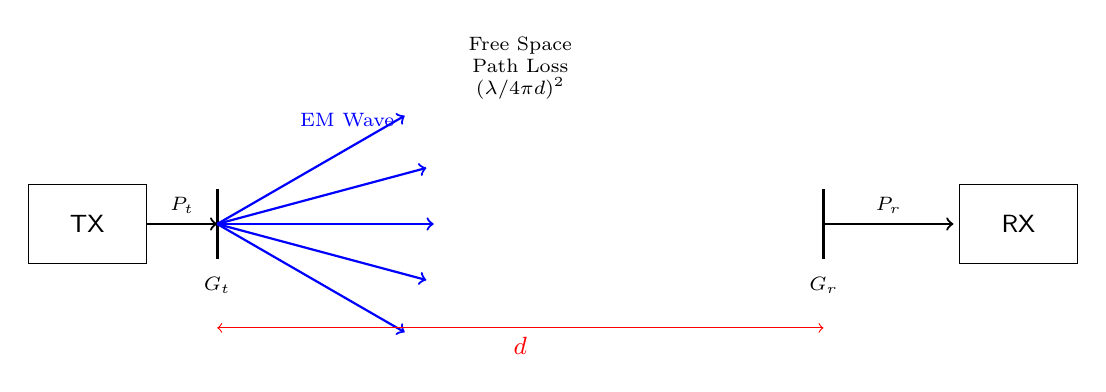
\begin{tikzpicture}[scale=1.1]
% Transmitter
\node[draw,rectangle,minimum width=1.5cm,minimum height=1cm,font=\sffamily\small] (tx) at (0,0) {TX};
\draw[thick,->] (tx.east) -- (1.5,0) node[midway,above,font=\scriptsize] {$P_t$};

% TX Antenna
\draw[very thick] (1.5,-0.4) -- (1.5,0.4);
\node[below,font=\scriptsize] at (1.5,-0.5) {$G_t$};

% Radiation
\foreach \angle in {-30,-15,0,15,30} {
  \draw[->,blue,thick] (1.5,0) -- +(\angle:2.5);
}
\node[blue,font=\scriptsize] at (3,1.2) {EM Wave};

% Distance
\draw[<->,red] (1.5,-1.2) -- (8.5,-1.2) node[midway,below,font=\small] {$d$};

% RX Antenna
\draw[very thick] (8.5,-0.4) -- (8.5,0.4);
\node[below,font=\scriptsize] at (8.5,-0.5) {$G_r$};

% Receiver
\draw[thick,->] (8.5,0) -- (10,0) node[midway,above,font=\scriptsize] {$P_r$};
\node[draw,rectangle,minimum width=1.5cm,minimum height=1cm,font=\sffamily\small] (rx) at (10.75,0) {RX};

% Path loss annotation
\node[font=\scriptsize,align=center] at (5,1.8) {Free Space\\Path Loss\\$(\lambda/4\pi d)^2$};
\end{tikzpicture}
\end{center}

\begin{keyconcept}
Antenna gain \textbf{adds} to the link budget (in dB), directly compensating for path loss. High-gain antennas enable long-distance communication by focusing power in the desired direction (TX) and increasing sensitivity (RX).
\end{keyconcept}

\section{Worked Example: Satellite Downlink Design}

\textbf{Scenario:} Design a geostationary satellite downlink for a 1~m ground station receiving Ku-band data.

\subsection*{Given Parameters}

\begin{tabular}{@{}ll@{}}
\toprule
\textbf{Parameter} & \textbf{Value} \\
\midrule
TX power & $P_t = 50$ W = 47 dBm \\
TX antenna (satellite dish) & $G_t = 35$ dBi \\
Distance (GEO orbit) & $d = 36{,}000$ km \\
Frequency (Ku-band) & $f = 12$ GHz \\
Wavelength & $\lambda = c/f = 0.025$ m \\
RX antenna diameter & $D_r = 1$ m \\
RX antenna efficiency & $\eta_{\text{ap}} = 0.65$ \\
System noise temperature & $T_s = 200$ K \\
Receiver bandwidth & $B = 5$ MHz \\
Required BER & $10^{-6}$ \\
\bottomrule
\end{tabular}

\subsection*{Step 1: Calculate RX Antenna Gain}

First, determine the physical aperture area:
\begin{equation}
A_{\text{phys}} = \pi \left(\frac{D_r}{2}\right)^2 = \pi \left(\frac{1}{2}\right)^2 = 0.785\ \text{m}^2
\end{equation}

Calculate effective aperture using efficiency:
\begin{equation}
A_e = \eta_{\text{ap}} \cdot A_{\text{phys}} = 0.65 \times 0.785 = 0.510\ \text{m}^2
\end{equation}

Convert to gain using Equation~\ref{eq:effective-aperture}:
\begin{equation}
G_r = \frac{4\pi A_e}{\lambda^2} = \frac{4\pi \times 0.510}{(0.025)^2} = 10{,}257\ (\text{linear}) = 40.1\ \text{dBi}
\end{equation}

\subsection*{Step 2: Calculate Free-Space Path Loss}

Using the FSPL formula:
\begin{equation}
L_{\text{FSPL}} = 20\log_{10}(d) + 20\log_{10}(f) + 92.45
\end{equation}

With $d$ in km and $f$ in MHz:
\begin{equation}
L_{\text{FSPL}} = 20\log_{10}(36{,}000) + 20\log_{10}(12{,}000) + 92.45 = 205.5\ \text{dB}
\end{equation}

\subsection*{Step 3: Calculate Received Signal Power}

Using the Friis equation (Equation~\ref{eq:friis-db}):
\begin{equation}
P_r = P_t + G_t + G_r - L_{\text{FSPL}}
\end{equation}
\begin{equation}
P_r = 47 + 35 + 40.1 - 205.5 = -83.4\ \text{dBm}
\end{equation}

\subsection*{Step 4: Calculate Noise Power}

The thermal noise power is:
\begin{equation}
N = kT_sB = (1.38 \times 10^{-23})(200)(5 \times 10^6) = 1.38 \times 10^{-14}\ \text{W}
\end{equation}

Converting to dBm:
\begin{equation}
N\ [\text{dBm}] = 10\log_{10}\left(\frac{1.38 \times 10^{-14}}{10^{-3}}\right) = -108.6\ \text{dBm}
\end{equation}

\subsection*{Step 5: Calculate Signal-to-Noise Ratio}

\begin{equation}
\text{SNR} = P_r - N = -83.4 - (-108.6) = 25.2\ \text{dB}
\end{equation}

\subsection*{Step 6: Determine Link Margin}

For QPSK with BER = $10^{-6}$, the required $E_b/N_0 \approx 10.5$ dB.

Assuming data rate $R_b = 2$ Mbps:
\begin{equation}
\frac{E_b}{N_0} = \text{SNR} + 10\log_{10}\left(\frac{B}{R_b}\right) = 25.2 + 10\log_{10}\left(\frac{5}{2}\right) = 25.2 + 4.0 = 29.2\ \text{dB}
\end{equation}

Link margin:
\begin{equation}
\text{Margin} = 29.2 - 10.5 = 18.7\ \text{dB}
\end{equation}

\begin{calloutbox}[colback=black!8!white,colframe=black]{Link Budget Summary}
\textbf{Result: Link closes with 18.7~dB margin}

This generous margin accommodates:
\begin{itemize}
\item Rain fade at Ku-band: $\sim$5--8 dB
\item Atmospheric absorption: $\sim$1--2 dB
\item Implementation losses: $\sim$2--3 dB
\item Pointing errors: $\sim$1--2 dB
\item Component aging and degradation
\end{itemize}

\textbf{Conclusion:} The 1~m ground station with 40~dBi gain is suitable for reliable 2~Mbps downlink reception. The high antenna gains (35~dBi TX, 40~dBi RX) compensate for the extreme 205.5~dB path loss at 36,000~km distance.
\end{calloutbox}

\section{Antenna Design by Frequency}

\subsubsection{VLF/LF (\textless{} 300 kHz)}\label{vlflf-300-khz}

\textbf{Challenge}: Wavelength \textgreater\textgreater{} practical
antenna size

\textbf{Solution}: - \textbf{Electrically small antennas} (length
\(\ll \lambda\)) - \textbf{Low efficiency} (most power lost in ohmic
resistance) - \textbf{Loading coils} to resonate (match reactance)

\textbf{Example}: 100 kHz (\$\textbackslash lambda\$ = 3000 m), 10 m
vertical monopole: - Radiation resistance: \textasciitilde0.1
\$\textbackslash Omega\$ - Loss resistance: \textasciitilde10
\$\textbackslash Omega\$ - Efficiency: \textasciitilde1\%

\begin{center}\rule{0.5\linewidth}{0.5pt}\end{center}

\subsubsection{HF/VHF (3-300 MHz)}\label{hfvhf-3-300-mhz}

\textbf{Sweet spot}: Antennas are practical size

\textbf{Common types}: - Dipole (\$\textbackslash lambda\$/2): 50 m @ 3
MHz, 1 m @ 150 MHz - Monopole (\$\textbackslash lambda\$/4): 25 m @ 3
MHz (vertical tower) - Yagi-Uda: TV reception (VHF channels)

\textbf{Efficiency}: 50-90\% (good conductors, minimal loss)

\begin{center}\rule{0.5\linewidth}{0.5pt}\end{center}

\subsubsection{UHF/SHF (300 MHz - 30
GHz)}\label{uhfshf-300-mhz---30-ghz}

\textbf{Miniaturization}: Antennas fit on PCBs

\textbf{Common types}: - Patch (microstrip): 3 cm
\$\textbackslash times\$ 3 cm @ 2.4 GHz - Slot: Waveguide-based (radar,
satellite) - Horn: Wideband, calibration standard

\textbf{Phased arrays become feasible}: Element spacing
\(d \sim \lambda/2\)

\textbf{Example}: 10 GHz, \(\lambda = 3\) cm
\$\textbackslash rightarrow\$ 1.5 cm spacing
\$\textbackslash rightarrow\$ 100 elements in 15 cm
\$\textbackslash times\$ 15 cm

\begin{center}\rule{0.5\linewidth}{0.5pt}\end{center}

\subsubsection{EHF/THz (30 GHz - 10 THz)}\label{ehfthz-30-ghz---10-thz}

\textbf{Challenges}: - \textbf{Fabrication tolerance}
(\$\textbackslash mu\$m precision required) - \textbf{Surface roughness
losses} (skin depth at THz \textasciitilde{} nm) - \textbf{Impedance
matching} difficult (high frequencies)

\textbf{Solutions}: - \textbf{On-chip antennas} (silicon, III-V
semiconductors) - \textbf{Photolithography} (THz: \textless100
\$\textbackslash mu\$m features) - \textbf{Lens-coupled antennas} (match
impedance to free space)

\textbf{Example}: 1.875 THz (AID protocol), \(\lambda = 160\)
\$\textbackslash mu\$m: - Dipole: 80 \$\textbackslash mu\$m (fabricated
via e-beam lithography) - Phased array: 40 \$\textbackslash mu\$m
spacing, 1024 elements in 40 mm \$\textbackslash times\$ 40 mm

\begin{center}\rule{0.5\linewidth}{0.5pt}\end{center}

\subsection{Antenna Measurements}\label{antenna-measurements}

\subsubsection{Anechoic Chamber}\label{anechoic-chamber}

\textbf{Facility for measuring radiation patterns}:

\begin{itemize}
\tightlist
\item
  \textbf{Absorber walls}: Eliminate reflections (simulate free space)
\item
  \textbf{Turntable}: Rotate antenna under test (AUT)
\item
  \textbf{Reference antenna}: Known gain/pattern
\item
  \textbf{Network analyzer}: Measure
  S\textbackslash textsubscript\{2\}\textbackslash textsubscript\{1\}
  (transmission) vs angle
\end{itemize}

\textbf{Far-field distance:}
\begin{equation}
d_{\text{far}} > \frac{2D^2}{\lambda}
\label{eq:far-field-distance}
\end{equation}
where $D$ is the largest antenna dimension (Fraunhofer region).

\textbf{Example:} 1 m dish @ 10 GHz ($\lambda = 0.03$ m) requires $d > 2 \times 1^2 / 0.03 = 67$ m (large chamber!)

\begin{center}
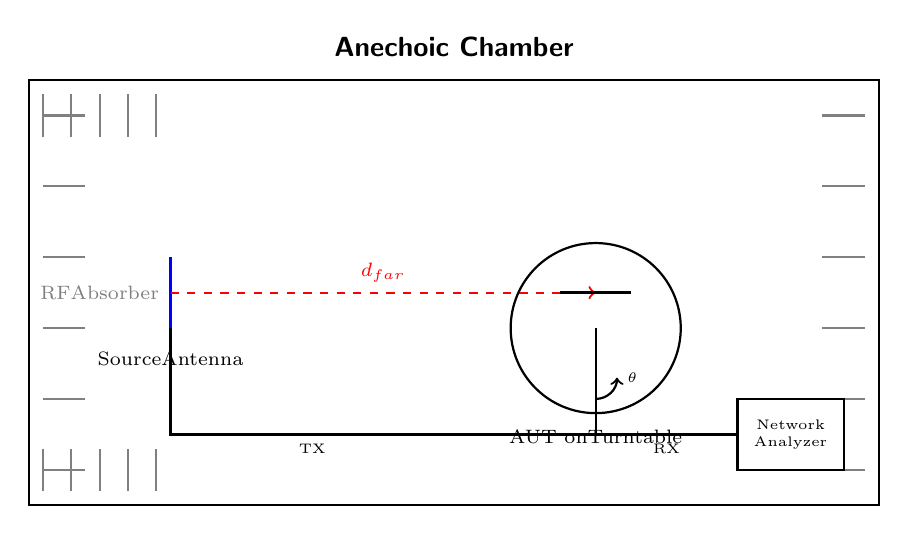
\begin{tikzpicture}[scale=0.9]
% Chamber walls
\draw[thick] (0,0) rectangle (12,6);
\node[above,font=\sffamily\bfseries] at (6,6.2) {Anechoic Chamber};

% Absorber material
\foreach \x in {0.2,0.6,1.0,1.4,1.8}{
  \draw[thick,gray] (\x,0.2) -- (\x,0.8);
  \draw[thick,gray] (\x,5.2) -- (\x,5.8);
}
\foreach \y in {0.5,1.5,2.5,3.5,4.5,5.5}{
  \draw[thick,gray] (0.2,\y) -- (0.8,\y);
  \draw[thick,gray] (11.2,\y) -- (11.8,\y);
}
\node[font=\scriptsize,gray] at (1,3) {RF\\Absorber};

% Transmit antenna (fixed)
\draw[very thick,blue] (2,2.5) -- (2,3.5);
\node[below,font=\scriptsize] at (2,2.3) {Source\\Antenna};

% Signal path
\draw[->,thick,red,dashed] (2,3) -- (8,3) node[midway,above,font=\scriptsize] {$d_{\text{far}}$};

% Antenna under test (AUT) on turntable
\draw[thick] (8,2.5) circle (1.2);
\draw[very thick,black] (7.5,3) -- (8.5,3);
\node[below,font=\scriptsize] at (8,1.2) {AUT on\\Turntable};
\draw[->,thick] (8,1.5) arc (270:360:0.3) node[right,font=\tiny] {$\theta$};

% Network analyzer
\draw[thick] (10,0.5) rectangle (11.5,1.5);
\node[font=\tiny,align=center] at (10.75,1) {Network\\Analyzer};

% Cables
\draw[thick] (2,2.5) -- (2,1) -- (10,1);
\draw[thick] (8,2.5) -- (8,1) -- (10,1);

% Labels for signals
\node[font=\tiny] at (4,0.8) {TX};
\node[font=\tiny] at (9,0.8) {RX};
\end{tikzpicture}
\end{center}

\subsubsection{Near-Field Scanning}\label{near-field-scanning}

\textbf{For electrically large antennas} (where far-field distance is
impractical):

\begin{enumerate}
\def\labelenumi{\arabic{enumi}.}
\tightlist
\item
  \textbf{Scan E/H fields} on planar/cylindrical/spherical surface near
  antenna
\item
  \textbf{FFT transform} to compute far-field pattern
\item
  \textbf{Smaller chamber} required (1-2 m)
\end{enumerate}

\begin{center}\rule{0.5\linewidth}{0.5pt}\end{center}

\subsubsection{Gain Measurement (Comparison Method)}

The comparison method determines antenna gain by measuring relative to a calibrated standard:

\textbf{Procedure:}
\begin{enumerate}
\item Measure received power with \textbf{standard gain horn} (calibrated): $P_{\text{std}}$
\item Replace with \textbf{antenna under test} (AUT): $P_{\text{AUT}}$
\item Compare powers using:
\end{enumerate}

\begin{equation}
G_{\text{AUT}}\ [\text{dBi}] = G_{\text{std}}\ [\text{dBi}] + (P_{\text{AUT}} - P_{\text{std}})\ [\text{dB}]
\label{eq:gain-comparison}
\end{equation}

This method eliminates the need to know absolute power levels or path loss, as both cancel in the comparison.

\subsection{Practical Design
Considerations}\label{practical-design-considerations}

\subsubsection{1. Matching Network}\label{matching-network}

\textbf{Goal}: Transform antenna impedance to 50\$\textbackslash Omega\$

\textbf{Techniques}: - \textbf{LC network}: Series/shunt
inductors/capacitors - \textbf{Quarter-wave transformer}:
\(Z_{\lambda/4} = \sqrt{Z_0 Z_{\text{ant}}}\) - \textbf{Stub matching}:
Open/short-circuited transmission line stubs

\textbf{Example}: Dipole (\(Z = 73 + j42.5\ \Omega\)) to
50\$\textbackslash Omega\$: - Add series capacitor to cancel reactance
(j42.5\$\textbackslash Omega\$) - Use transformer to match
73\$\textbackslash Omega\$ to 50\$\textbackslash Omega\$

\begin{center}\rule{0.5\linewidth}{0.5pt}\end{center}

\subsubsection{2. Balun (Balanced-Unbalanced
Transformer)}\label{balun-balanced-unbalanced-transformer}

\textbf{Problem}: Coaxial cable (unbalanced) feeding dipole (balanced)
\$\textbackslash rightarrow\$ Common-mode currents on outer shield
(pattern distortion)

\textbf{Solution}: Balun isolates antenna from feedline

\textbf{Types}: - \textbf{Choke balun}: Coil of coax (high impedance to
common-mode) - \textbf{Sleeve balun}: \$\textbackslash lambda\$/4 sleeve
over coax - \textbf{Transformer balun}: 1:1 or 4:1 turns ratio (ferrite
core)

\begin{center}\rule{0.5\linewidth}{0.5pt}\end{center}

\subsubsection{3. Environmental Effects}\label{environmental-effects}

\paragraph{Ground Plane}\label{ground-plane}

\begin{itemize}
\tightlist
\item
  \textbf{Monopole requires ground plane} (acts as mirror image)
\item
  \textbf{Poor ground} (dry soil, concrete)
  \$\textbackslash rightarrow\$ Reduced efficiency
\item
  \textbf{Elevated radials} (4-8 wires, \$\textbackslash lambda\$/4
  length) improve performance
\end{itemize}

\paragraph{Nearby Objects}\label{nearby-objects}

\begin{itemize}
\tightlist
\item
  \textbf{Metal structures}: Detune antenna (shift resonance), reflect
  energy
\item
  \textbf{Human body}: Lossy dielectric (especially at cellular
  frequencies) \$\textbackslash rightarrow\$ Detuning, absorption
\item
  \textbf{Solution}: Antenna placement away from body (smartphones:
  top/bottom), adaptive matching
\end{itemize}

\begin{center}\rule{0.5\linewidth}{0.5pt}\end{center}

\section{Real-World Applications}

This section highlights specific antenna implementations in operational systems.

\subsection{Satellite Communications}

\subsubsection{GPS (L1 Band, 1.575 GHz)}
\begin{itemize}
\item \textbf{Satellite antenna:} Phased array, 13~dBi gain, RHCP
\item \textbf{Transmit power:} 27~W (14.3~dBm effective EIRP)
\item \textbf{User antenna:} Patch or helical, 3--5~dBi, RHCP
\item \textbf{Link budget:} Operates with received power $\sim$-130~dBm (extremely weak signal, requires correlation processing)
\end{itemize}

\subsubsection{Direct-to-Home Satellite TV (Ku-band, 12 GHz)}
\begin{itemize}
\item \textbf{Satellite antenna:} Multiple spot beams, 35--40~dBi
\item \textbf{User dish:} 45--60~cm diameter, 35--38~dBi
\item \textbf{Polarization:} Linear (H/V) or circular for frequency reuse
\item \textbf{Key requirement:} Precise pointing (beamwidth $\sim$2--3$°$)
\end{itemize}

\subsection{Terrestrial Wireless}

\subsubsection{5G Massive MIMO Base Station}
\begin{itemize}
\item \textbf{Configuration:} 64--256 element array (3.5~GHz)
\item \textbf{Element spacing:} $\lambda/2 = 4.3$ cm
\item \textbf{Array gain:} 24--28~dBi with beamforming
\item \textbf{Capability:} Electronic beam steering, spatial multiplexing for multiple users simultaneously
\end{itemize}

\subsubsection{WiFi 6E (6 GHz)}
\begin{itemize}
\item \textbf{Access point:} Multiple patch antennas, 5--8~dBi per antenna
\item \textbf{MIMO configuration:} 4$\times$4 or 8$\times$8
\item \textbf{Client devices:} Integrated patch/PIFA, 2--4~dBi
\item \textbf{Polarization diversity:} Improves link reliability in multipath
\end{itemize}

\subsection{Radar Systems}

\subsubsection{Automotive Radar (77 GHz)}
\begin{itemize}
\item \textbf{Antenna:} Planar phased array on PCB
\item \textbf{Elements:} 12--16 patch antennas
\item \textbf{Gain:} 20--25~dBi
\item \textbf{Beamwidth:} Narrow elevation (15$°$), wide azimuth (30$°$) for lane coverage
\item \textbf{Application:} Adaptive cruise control, collision avoidance
\end{itemize}

\subsubsection{Weather Radar (S-band, 3 GHz)}
\begin{itemize}
\item \textbf{Antenna:} Parabolic reflector, 3--8~m diameter
\item \textbf{Gain:} 40--50~dBi
\item \textbf{Polarization:} Dual-pol (H+V) for precipitation classification
\item \textbf{Scanning:} Mechanical rotation for 360$°$ coverage
\end{itemize}

\subsection{Emerging Technologies}

\subsubsection{Terahertz Communications (300 GHz)}
\begin{itemize}
\item \textbf{On-chip antennas:} Integrated with III-V semiconductors
\item \textbf{Dimensions:} $\sim$100--500~$\mu$m
\item \textbf{Phased arrays:} 64--1024 elements for high gain
\item \textbf{Challenge:} Fabrication tolerance, surface roughness losses
\item \textbf{Application:} Ultra-high bandwidth wireless backhaul
\end{itemize}

\section{Summary: Key Antenna Formulas}

{\def\LTcaptype{} % do not increment counter
\begin{longtable}[]{@{}
  >{\raggedright\arraybackslash}p{(\linewidth - 4\tabcolsep) * \real{0.4074}}
  >{\raggedright\arraybackslash}p{(\linewidth - 4\tabcolsep) * \real{0.3333}}
  >{\raggedright\arraybackslash}p{(\linewidth - 4\tabcolsep) * \real{0.2593}}@{}}
\toprule\noalign{}
\begin{minipage}[b]{\linewidth}\raggedright
Parameter
\end{minipage} & \begin{minipage}[b]{\linewidth}\raggedright
Formula
\end{minipage} & \begin{minipage}[b]{\linewidth}\raggedright
Units
\end{minipage} \\
\midrule\noalign{}
\endhead
\bottomrule\noalign{}
\endlastfoot
\textbf{Gain} & \(G = \eta_{\text{ant}} \cdot D\) & Linear or dBi \\
\textbf{Effective aperture} & \(A_e = \frac{G\lambda^2}{4\pi}\) &
m\textbackslash textsuperscript\{2\} \\
\textbf{Beamwidth (aperture)} & \(\theta \approx 70\lambda/D\) &
Degrees \\
\textbf{Directivity (narrow beam)} &
\(D \approx 41253/(\theta_E \theta_H)\) & Linear \\
\textbf{Friis equation} & \(P_r = P_t G_t G_r (\lambda/4\pi d)^2\) &
Watts \\
\textbf{FSPL} & \(L = 20\log(d) + 20\log(f) + 92.45\) & dB \\
\textbf{Radiation resistance (dipole)} & \(R_r = 73\ \Omega\) & Ohms \\
\textbf{SWR} & \(\text{SWR} = (1+|\Gamma|)/(1-|\Gamma|)\) & Ratio \\
\end{longtable}
}

\begin{center}\rule{0.5\linewidth}{0.5pt}\end{center}

\section{Summary}

\subsection{Key Antenna Performance Comparison}

\begin{center}
\begin{tabular}{@{}lcccc@{}}
\toprule
\textbf{Antenna Type} & \textbf{Gain} & \textbf{Beamwidth} & \textbf{Bandwidth} & \textbf{Application} \\
\midrule
Isotropic (reference) & 0 dBi & 360$°$ & -- & Theoretical \\
Dipole ($\lambda$/2) & 2.15 dBi & 78$°$ & 2--5\% & VHF/UHF base \\
Monopole ($\lambda$/4) & 5.15 dBi & 30$°$ & 2--5\% & Mobile/vehicle \\
Patch & 6--9 dBi & 70--90$°$ & 2--5\% & GPS, cellular \\
Yagi & 10--15 dBi & 30--60$°$ & 5--10\% & TV, point-to-point \\
Parabolic dish (1m@10GHz) & 40 dBi & 2$°$ & 10--20\% & Satellite \\
Phased array (64 elem) & 18--24 dBi & Steerable & 10--20\% & Radar, 5G \\
\bottomrule
\end{tabular}
\end{center}

\subsection{Design Trade-offs}

\textbf{Advantages of high-gain antennas:}
\begin{itemize}
\item Increased link range (every 3~dB gain doubles effective range in power-limited scenarios)
\item Improved signal-to-noise ratio
\item Interference rejection from other directions
\end{itemize}

\textbf{Disadvantages of high-gain antennas:}
\begin{itemize}
\item Narrow beamwidth requires precise pointing
\item Larger physical size (for aperture antennas)
\item Higher cost and complexity
\item Reduced coverage area
\end{itemize}

\textbf{Best suited for:}
\begin{itemize}
\item \textbf{High gain:} Long-distance links (satellite, point-to-point)
\item \textbf{Omnidirectional:} Mobile users, broadcast (WiFi, cellular base)
\item \textbf{Phased arrays:} Dynamic beam steering (radar, 5G, interference mitigation)
\end{itemize}

\section{Further Reading}

\textbf{Foundation topics:}
\begin{itemize}
\item \textbf{Electromagnetic Spectrum:} Frequency-dependent antenna design considerations
\item \textbf{Maxwell's Equations \& Wave Propagation:} Fundamental radiation mechanism
\item \textbf{Power Density \& Field Strength:} Near-field and far-field relationships
\end{itemize}

\textbf{Link budget analysis:}
\begin{itemize}
\item \textbf{Free-Space Path Loss (FSPL):} Distance-dependent propagation loss
\item \textbf{Signal-to-Noise Ratio (SNR):} How antenna gain improves SNR
\item \textbf{Complete Link Budget Analysis:} End-to-end system design
\end{itemize}

\textbf{Advanced topics:}
\begin{itemize}
\item \textbf{Wave Polarization:} Detailed polarization theory and applications
\item \textbf{Propagation Modes:} Ground-wave, sky-wave, line-of-sight
\item \textbf{Multipath \& Fading:} Antenna diversity, MIMO systems
\item \textbf{AID Protocol Case Study:} THz phased array example (1.875~THz, 40~dB gain)
\end{itemize}
